% Dirichlet Processes
\lecture{Dirichlet Process Priors for Mixture Models}{Dirichlet}


\begin{frame}
	\frametitle{Mixture Models}
	\begin{itemize}
		\item A common strategy when faced with complex multi-modal data is to fit a \emph{mixture model}.
		\item In general:
		\[
			p(\bx) = \sum_{k=1}^K P(k)p(\bx|k)
		\]
		\item Where each component $p(\bx|k)$ is some simple density, e.g. Gaussian
		\item Within this model, we must know $K$ \emph{a-priori}
		\item Can do inference with Expectation-Maximisation, Variational Bayes, Gibbs Sampling, etc
		\item Generative process for $N$ data points:
		\begin{itemize}
			\item For each datapoint, $n$:
			\begin{itemize}
				\item Sample a component ($k$) according to $P(k)$.
				\item Sample $\bx_n\sim p(\bx_n|k)$
			\end{itemize}
		\end{itemize}
	\end{itemize}
\end{frame}

\begin{frame}
	\frametitle{Gibbs sampling for mixture models}
	\begin{itemize}
		\item Assume that the $k$th mixture component has parameters $\theta_k$.
		\item Define binary variables $z_{nk}$ where $z_{nk}=1$ if $n$th object is \emph{in} $k$th component and zero otherwise.
		\item Define $\pi_k = P(k)$.
		\item Define prior density on $\theta_k$: $p(\theta_k)$.
		\item For each iteration:
		\begin{itemize}
			\item Sample each $\theta_k$ from $p(\theta_k|\ldots) \propto p(\theta_k)\prod_n p(\bx_n|\theta_k)^{z_{nk}}$\\
			\item For each object $n$:
			\begin{itemize}
				\item Remove from its current component.
				\item Sample a new component: $P(z_{nk}=1|\ldots)\propto \pi_k p(\bx_n|\theta_k)$
			\end{itemize}
		\end{itemize}
	\end{itemize}
\end{frame}

\begin{frame}
	\frametitle{Being Bayesian}
	\begin{itemize}
		\item We should treat $\boldsymbol\pi = [\pi_1,\ldots,\pi_K]^T$ as a random variable.
		\item A suitable prior density is the Dirichlet:
		\[
			p(\boldsymbol\pi_k)  = \frac{\Gamma(\sum_k \beta)}{\prod_k \Gamma(\beta)}\prod_k \pi_k^{\beta_k-1}
		\]
		\item (from now on, we'll assume $\beta_k = \alpha/K~~\forall k$)
		\item<2->We will also assume that (\emph{a-priori}) the number of objects in each cluster ($c_k = \sum_n z_{nk}$) is multinomial with parameter $\bpi$:
		\[
			p(\mathbf{c}|\bpi) \propto \prod_k \pi_k^{c_k}
		\]
	\end{itemize}
\end{frame}

\begin{frame}
	\frametitle{Being Bayesian}
	\begin{itemize}
		\item We can now compute the posterior density for $\bpi$. It's another Dirichlet:
		\[
			p(\bpi|\mathbf{c},\alpha) =  \frac{\Gamma(\sum_k \alpha/K+c_k)}{\prod_k \Gamma(\alpha/K+c_k)}\prod_k \pi_k^{\alpha/K+c_k-1}
		\]
		\item<2->We can now also compute the probablity that some new observation would be placed in class $j$:
		\begin{eqnarray}
			\nonumber P(z_{*j} &=& 1|\mathbf{c},\alpha) = \int p(z_{*j}=1|\bpi)p(\bpi|\mathbf{c},\alpha)~d\bpi\\
			\nonumber &=& \int \pi_j p(\bpi|\mathbf{c},\alpha)\\
			\nonumber &=& \frac{c_j + \alpha/K}{\alpha + \sum_k c_k}
		\end{eqnarray}
		\item<2-> (Need to know that $\Gamma(z+1) = z\Gamma(z)$)
	\end{itemize}
\end{frame}

\begin{frame}
	\frametitle{Gibbs sampling again}
	\begin{itemize}
		\item Going back to our Gibbs sampling, we can replace $\pi_k$ with this expression:
		\[
			P(z_{nk}=1|\ldots)\propto \frac{c_k + \alpha/K}{\alpha + \sum_j c_j} p(\bx_n|\theta_k)
		\]
		\item Where the point being sampled shouldn't appear in any $c_j$ (i.e. $\sum_j c_j = N-1$)
	\end{itemize}
\end{frame}

\begin{frame}
	\frametitle{Sampling from the prior}
	\begin{itemize}
		\item We can ignore the data $\bx_n$ for a while and just sample partitions from this prior:
		\item Start with N objects, all in one cluster.
		\item For each iteration:
		\begin{itemize}
			\item For each object $n$:
			\begin{itemize}
				\item Remove from component it is in and re-assign with probability:
				\[
					P(z_{nk} = 1|\ldots) = \frac{c_k + \alpha/K}{\alpha + \sum_j c_k}
				\]
			\end{itemize}
		\end{itemize}
	\end{itemize}
\end{frame}

\begin{frame}
	\frametitle{Sampling from the prior}
	\begin{figure}[tbh]
		\centering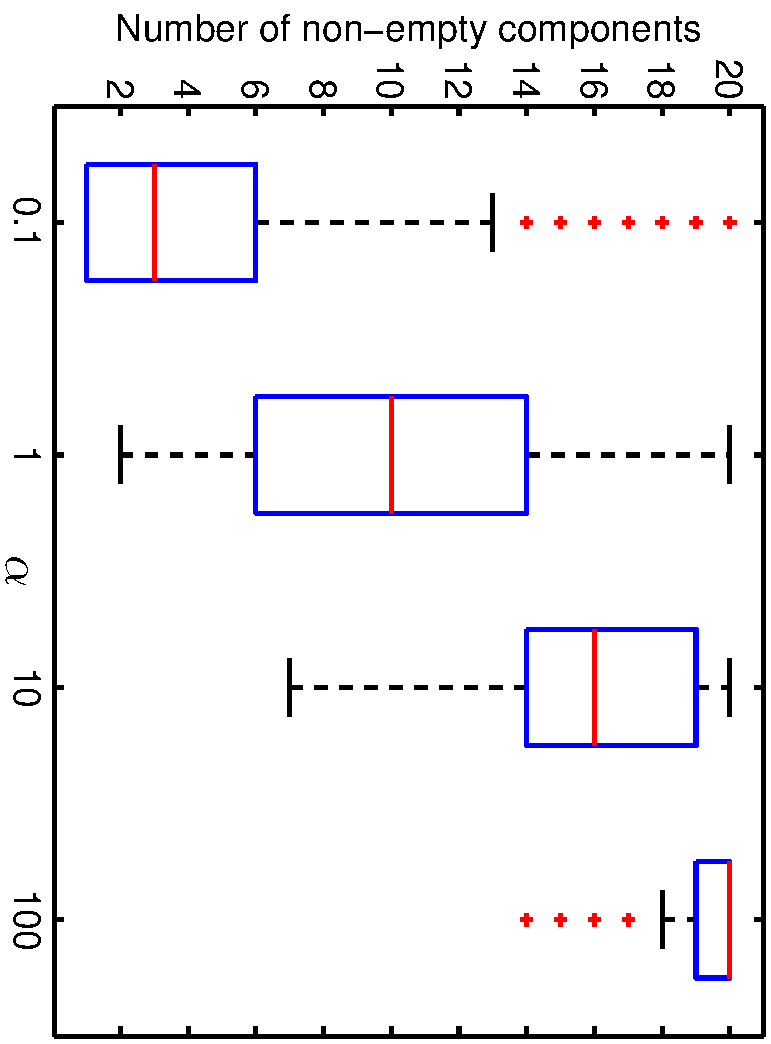
\includegraphics[height=0.8\linewidth,angle=90]{DPfixed.pdf}
		\centering\caption{\label{fig:dpfixed}Number of non-empty components as $\alpha$ is increased. $N=100$ and $K=20$. $\alpha$ controls how clustered the data are. Low $\alpha$ gives few populated clusters. Note: could have done this by sampling $\bpi$ and then sampling from $\bpi$)}
	\end{figure}
\end{frame}

\begin{frame}
	\frametitle{$K\rightarrow \infty$}
	\begin{itemize}
		\item What if we don't want to fix $K$?
		\item i.e. set $K=\infty$.
		\[
		P(Z_{nk}=1|\ldots) = \frac{c_k + \alpha/K}{\alpha + \sum_j c_j} = \frac{c_k}{\alpha + \sum_j c_j}
		\]
		\item This is the probability for one of the \emph{finite} number of clusters that are currently occupied.
		\item<2-> The probability of assigning to one of the \emph{infinite} number of unoccupied clusters must be:
		\[
		P(Z_{nk*}=1|\ldots) = 1 - \sum_k \frac{c_k}{\alpha + \sum_j c_j} = \frac{\alpha}{\alpha + \sum_j c_j}
		\]
		\item<3->A nice paper describing this: \href{http://www.gatsby.ucl.ac.uk/~edward/pub/inf.mix.nips.99.pdf}{Rasmussen 2000}
	\end{itemize}
\end{frame}

\begin{frame}
	\frametitle{Sampling from the $K=\infty$ prior}
	\begin{itemize}
		\item Start with $N$ objects all in one cluster
		\item For each iteration:
		\begin{itemize}
			\item For each object $n$:
			\begin{itemize}
				\item Remove from current component (if it leaves an empty component, delete it)
				\item Re-assign according to:
				\[
					P(z_{nk}=1|\ldots) = \left\{ \begin{array}{ll}
						\frac{c_k}{\alpha + \sum_j c_j} & \mbox{$k$ currently occupied}\\
						\frac{\alpha}{\alpha + \sum_j c_j} & \mbox{new $k$}
					\end{array}\right.
				\]
				\item if object in a new component, create one.
			\end{itemize}
		\end{itemize}
		\item<2->The prior we are sampling from is a \emph{Dirichlet Process}
	\end{itemize}
\end{frame}

\begin{frame}
	\frametitle{Sampling from the $K=\infty$ prior}
	\begin{figure}[tbh]
		\centering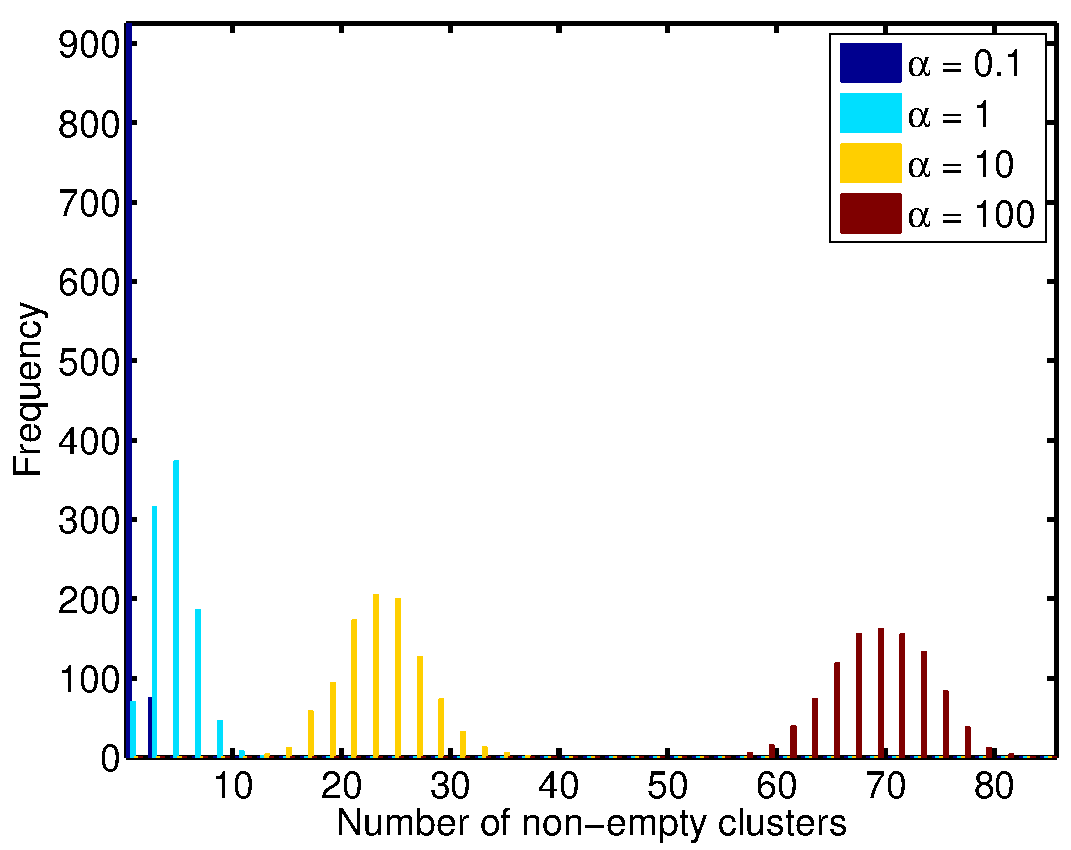
\includegraphics[width=0.8\linewidth]{DPbars.pdf}
		\centering\caption{\label{fig:DPbars}Number of non empty clusters as $\alpha$ is varied. $1000$ samples for $N=100$ objects.}
	\end{figure}
\end{frame}

\begin{frame}
	\frametitle{Including data}
	\begin{itemize}
		\item In general, we want to fit the model to objects $\bx_n$.
		\item Assume each component has parameters $\theta_k$.
		\item Assume a likelihood $p(\bx_n|\theta_k)$ and a prior $p(\theta_k)$
		\item<2->Gibbs sampling:
		\begin{itemize}
			\item Given a current clustering $\bZ$ and parameters $\theta_1,\ldots,\theta_k$
			\item For each object $\bx_n$ in each iteration:
			\begin{itemize}
				\item Remove $\bx_n$ from the model (might require deleting a component).
				\item Re-assign with probabilities:
				\[
					P(z_{nk}=1|\bx_n,\ldots)\propto \left\{\begin{array}{ll}
						c_k p(\bx_n|\theta_k) & \mbox{$k$ currently occupied}\\
						\alpha \int p(\bx_n|\theta)p(\theta)~d\theta & \mbox{new $k$}
					\end{array}\right.
				\]
				\item Sample $\theta_k$ for each component:
				\[
				p(\theta_k|\ldots)\propto p(\theta_k)\prod_n p(\bx_n|\theta_k)^{z_{nk}}
				\]
			\end{itemize}
		\end{itemize}
		\item<3->If everything conjugate, can integrate $\theta_k$ out completely (better convergence).
	\end{itemize}
\end{frame}
\begin{frame}
	\frametitle{\ac{CRP}}
	\begin{itemize}
		\item A popular way of thinking about DPs is via the `Chinese Restaurant Process'
		\item Prior:
		\begin{itemize}
			\item $N$ people enter a Chinese Restaurant with infinite tables.
			\item The first person sits at the first table.
			\item The $n$th person sits at an occupied table with probability proportional to the number of people already at the table, or a new table with probability proportional to $\alpha$.
		\end{itemize}
		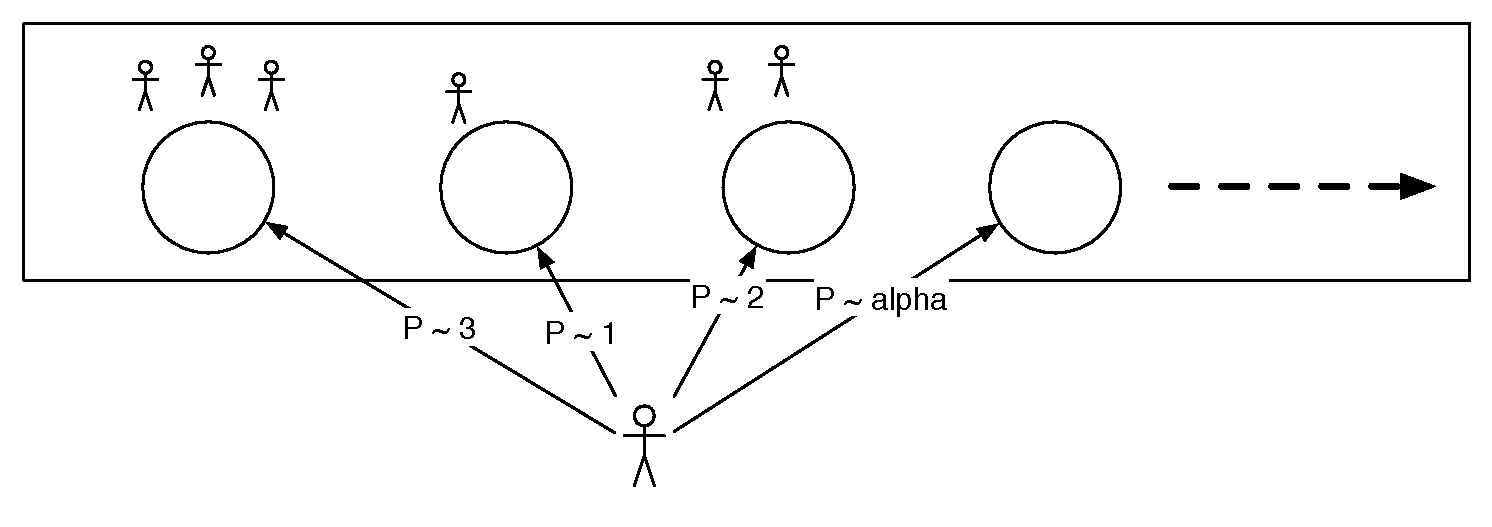
\includegraphics[width=\linewidth]{CRP.pdf}		
	\end{itemize}
\end{frame}

\begin{frame}
	\frametitle{\ac{CRP}}
	\begin{itemize}
		\item With data:
		\begin{itemize}
			\item Each table has one dish. Table choice also depends on dish preference.
			\item Table dishes updated according to preference of people at table (here the analogy starts(!) to get a bit tenuous)
		\end{itemize}
		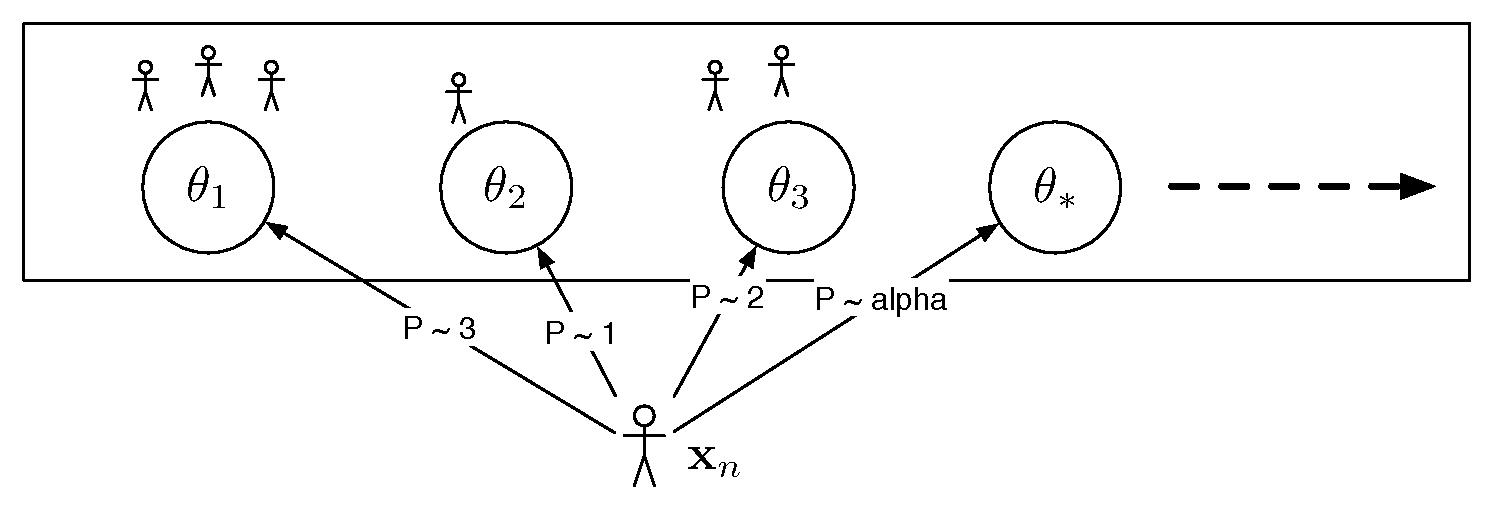
\includegraphics[width=\linewidth]{CRP2.pdf}
	\end{itemize}
\end{frame}

\begin{frame}
	\frametitle{Example}
	\begin{figure}[tbh]
		\centering\includegraphics<1>[width=0.7\linewidth]{CRP_data.pdf}
		\centering\includegraphics<2>[width=0.7\linewidth]{CRP_sim.pdf}
		\centering\includegraphics<3>[width=0.7\linewidth]{CRP_K.pdf}
		\centering\caption{\label{fig:CRP_example}Example output from CRP with Gibbs sampling. The data has three clusters. Visualising the $\theta_k$ is impossible, but we can look at the probablility that two objects are in the same cluster, and the number of clusters. (Data are sorted)}
	\end{figure}
\end{frame}

\begin{frame}
	\frametitle{Some practical tips}
	\begin{itemize}
		\item This works much better with conjugate models.
		\item Making it work on real problems is hard.
		\item It's not magic.
		\begin{itemize}
			\item Avoid specifying how many clusters there are\ldots
			\item \ldots but have to quite precisely speciy what a cluster looks like.
		\end{itemize}
		\item How to interpret the output?
		\begin{itemize}
			\item Great for things where the clustering is the \emph{input} to something else
		\end{itemize}
	\end{itemize}
\end{frame}
